\begin{figure*}[t]
\centering
% src: fig/abc_closeups.png by scripts/paper_figures_abc.py; regions: docs/paper/fig_abc_fig6c_regions.json; leads: docs/final-campaign-nov13.md (Visual comparison)
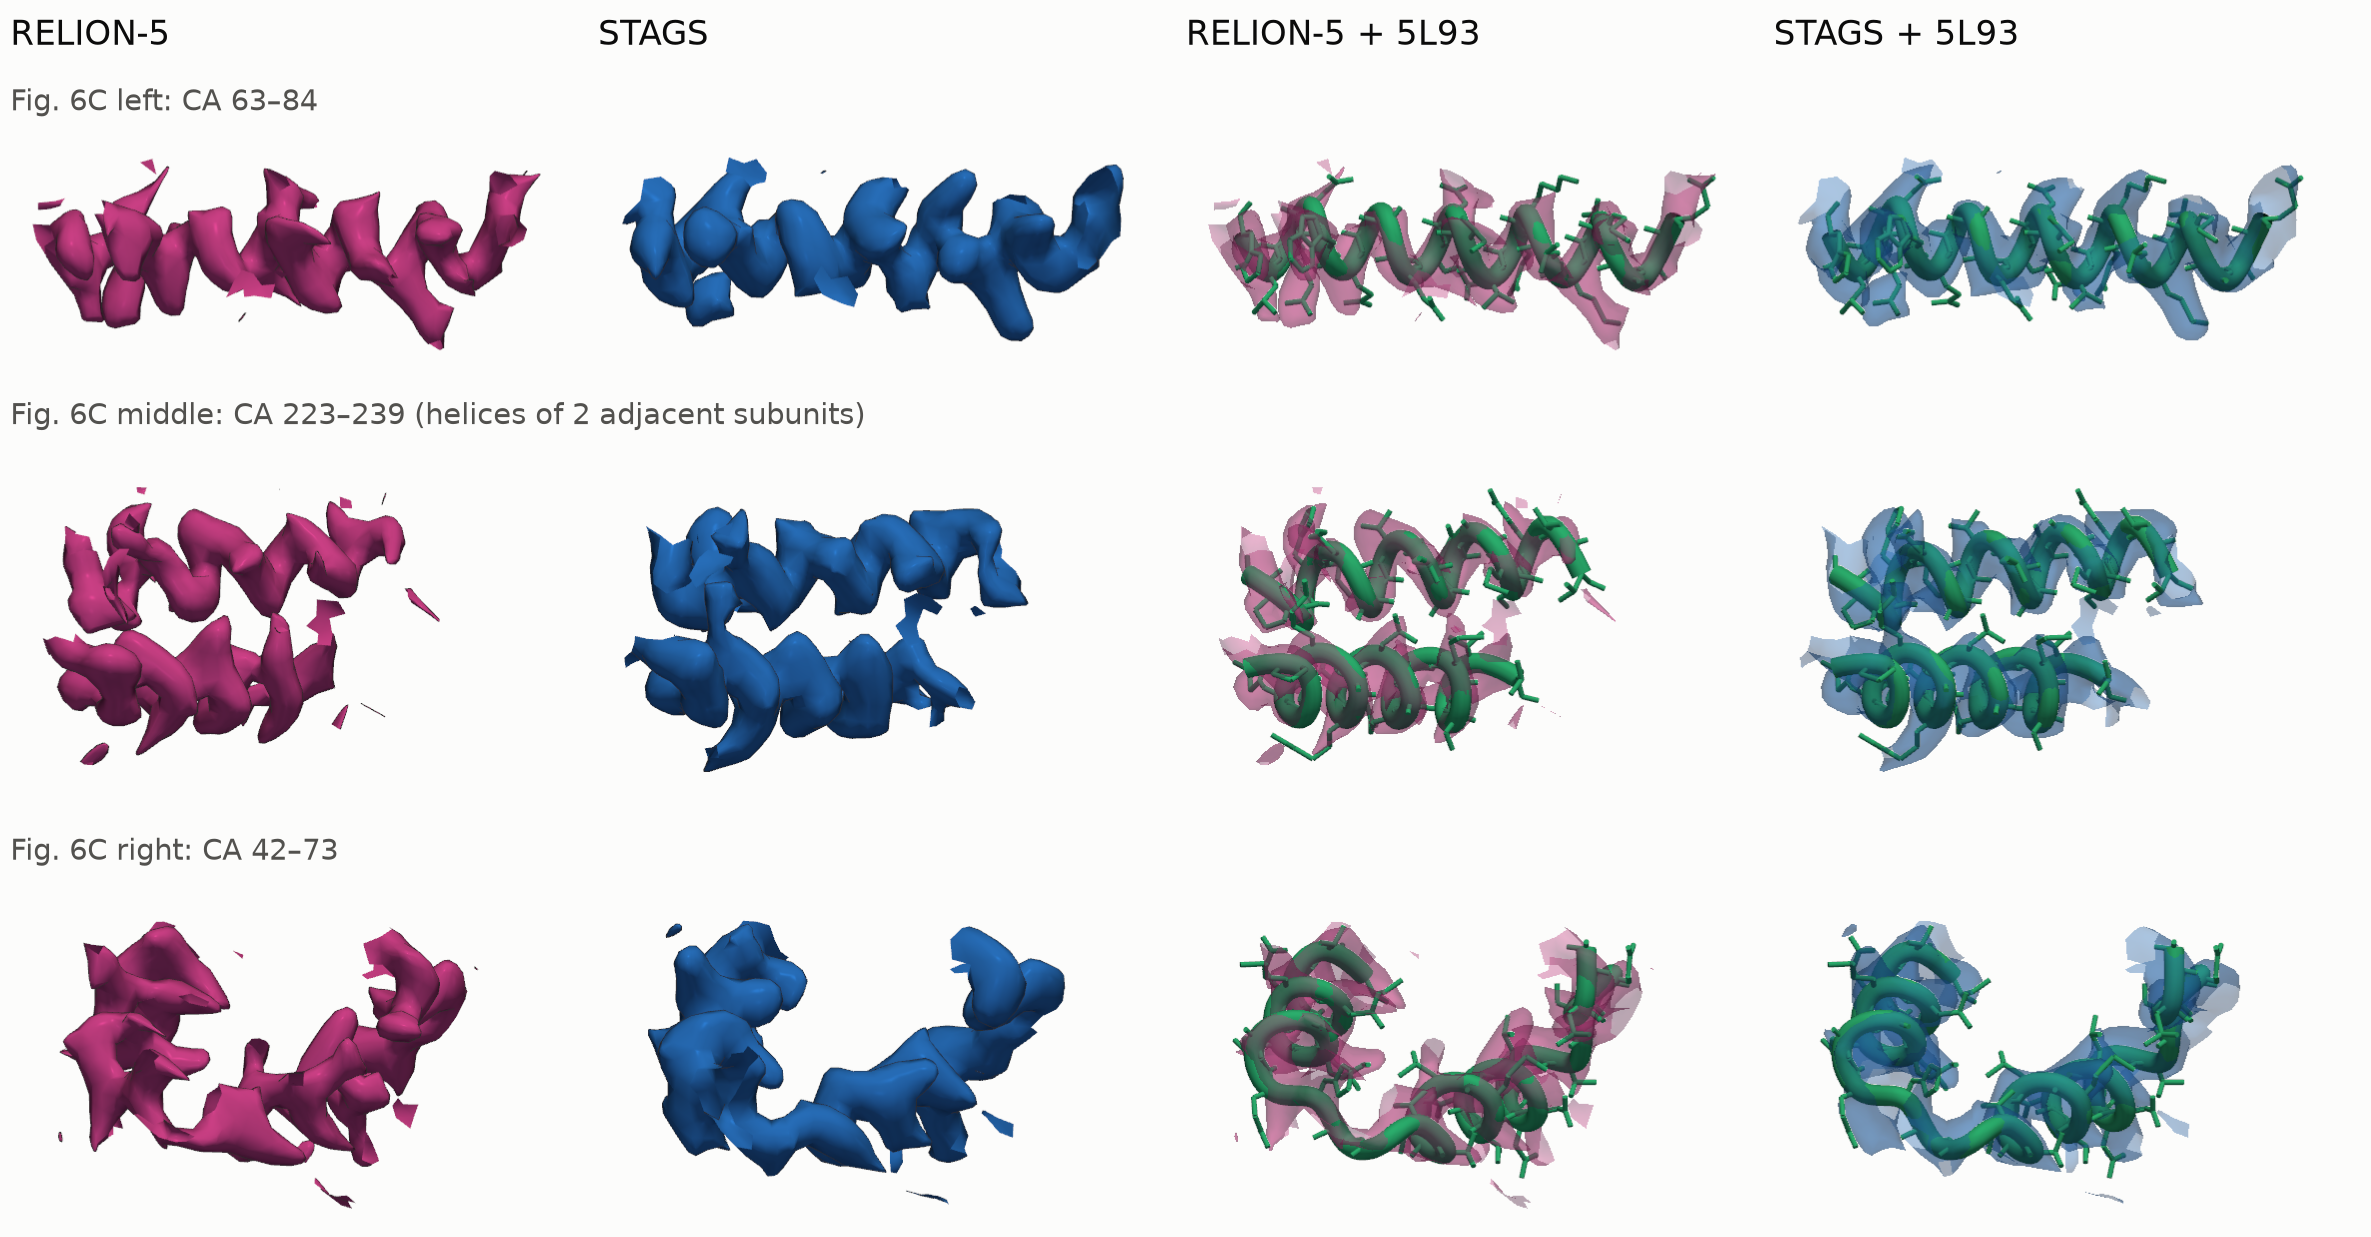
\includegraphics[width=0.92\textwidth]{fig/abc_closeups.png}
\caption{\textbf{Close-ups of the three regions shown in RELION-5's Fig.~6C~\cite{burt2024relion5}.}
Columns: RELION-5 polished map, STAGS, then each map translucent over the 5L93 model.
Rows: CA residues 63--84 (helix~4); 223--239 of two adjacent subunits; 42--73 (end of helix~2 to the start of helix~4).
The published figure does not list its regions; we recovered them by a joint silhouette match of 5L93 atoms and RELION density to the published panels, with leads of 1.59, 0.71 and 0.46\,px over the next distinct region, so the bottom row is the least certain.
Same filtering and threshold as \cref{fig:views}, zoned 2.5\,\AA\ around the shown residues, identical camera per row.}
\label{fig:closeups}
\end{figure*}
